\documentclass[letterpaper,12pt]{exam}

\usepackage{ge13}
\usepackage{comment}
\usepackage{booktabs}
\usepackage{hyperref}
\urlstyle{rm}   % change fonts for url's (from Chad Jones)
\hypersetup{
    colorlinks=true,        % kills boxes
    allcolors=blue,
    pdfsubject={NYU Stern course GB 2303, Global Economy},
    pdfauthor={Dave Backus @ NYU},
    pdfstartview={FitH},
    pdfpagemode={UseNone},
%    pdfnewwindow=true,      % links in new window
%    linkcolor=blue,         % color of internal links
%    citecolor=blue,         % color of links to bibliography
%    filecolor=blue,         % color of file links
%    urlcolor=blue           % color of external links
% see:  http://www.tug.org/applications/hyperref/manual.html
}

\newcommand{\NX}{\mbox{\em NX\/}}
\newcommand{\POP}{\mbox{\em POP\/}}
\renewcommand{\log}{\ln}

\usepackage{float}
\restylefloat{table}

\def\ClassName{The Global Economy}
\def\Category{David Backus}
\def\HeadName{Practice Midterm Examination 1}

\printanswers

\begin{document}
\parindent = 0.0in
\parskip = \bigskipamount
\thispagestyle{empty}%
\Head

\centerline{\large \bf \HeadName}%
%\centerline{March 9, 2005}
\centerline{Revised:  \today}

\bigskip
You have 90 minutes to complete this exam.  Please answer each
question in the space provided. You may consult one page of notes
and a calculator, but devices capable of wireless transmission are
prohibited.

I understand that the honor code applies: I will not lie, cheat,
or steal to gain an academic advantage, or tolerate those who do.

\begin{flushright}
\rule{4in}{0.5pt} \\ (Name and Signature)
\end{flushright}

{\it Note:  These questions come from old exams,
so the topics and numbers may be out of date.
But be assured:  good analysis lasts forever.}  \\

\begin{figure}[h]
    \centering
    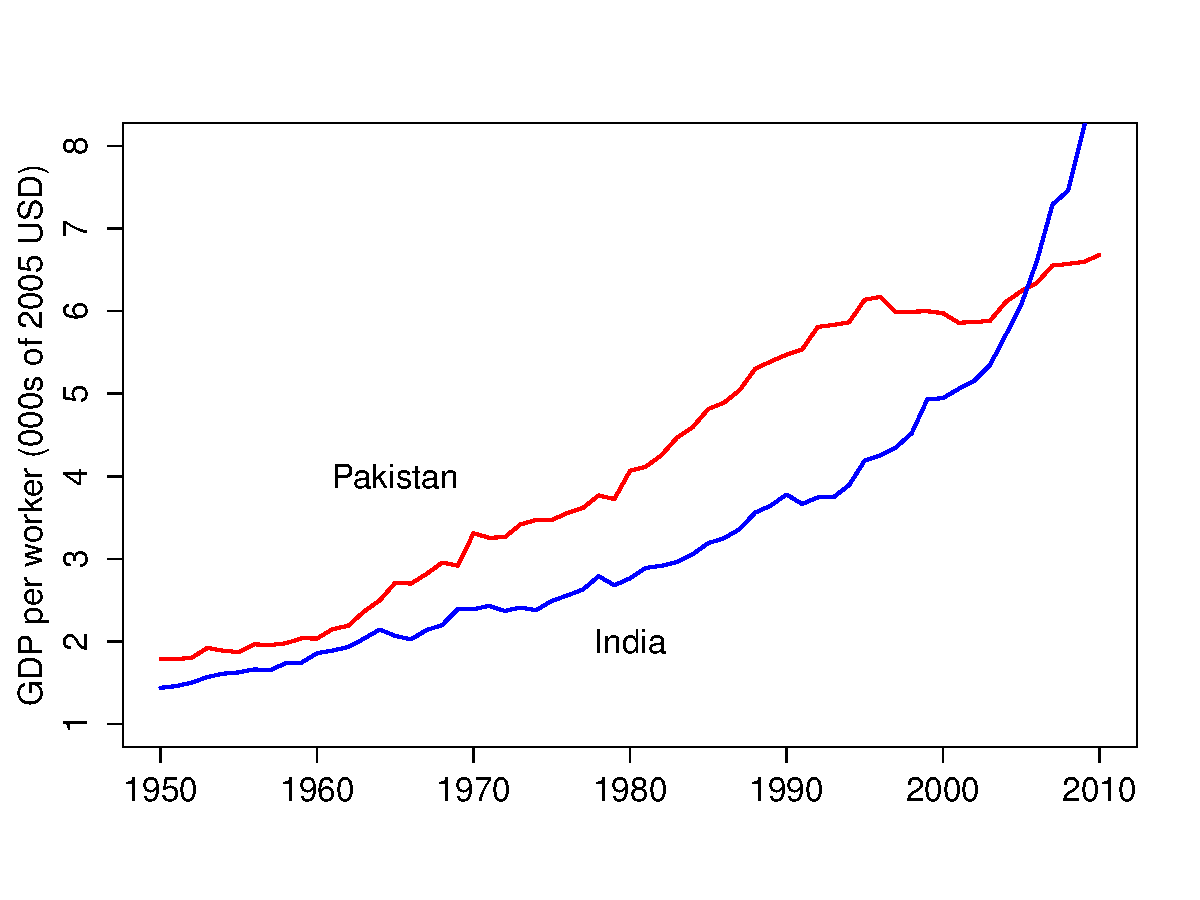
\includegraphics[scale=0.6]{PAKIND_s13_YL.pdf}
    \caption{GDP Per Worker in Pakistan and India.}
    \label{fig:pakistan}
\end{figure}

\begin{table}[h]
    \centering
    \tabcolsep = 0.3in
    \begin{tabular}{lrrr}
    \toprule
    & India & \multicolumn{2}{c}{Pakistan}  \\
    \cmidrule(r){2-2} \cmidrule{3-4}
    Year     &  $Y/L$ &  $ Y/L $   &  $K/L$   \\
    \midrule
    1990 &  3.780   &   5.473  &   9.040   \\
    2010 &  9.010   &   6.681  &   10.577  \\
    \bottomrule
    \end{tabular}
    \caption{Aggregate data for Pakistan and India.
    The numbers are thousands of 2005 US dollars.
    Source:  Penn World Table, Version 7.1.}
    \label{tab:pakistan}
\end{table}

\begin{table}[h]
    \centering
    \tabcolsep = 0.2in
    \begin{tabular}{lcc}
    \toprule
    & {Pakistan} & India \\
    \midrule
    Voice and accountability	& 26.3 & 59.2  \\
    Political stability	        & 0.5  & 12.7 \\
    Govt effectiveness	        & 22.3 & 54.5 \\
    Regulatory quality	        & 29.9 & 40.3 \\
    Rule of law		            & 20.7 & 52.6 \\
    Control of corruption	    & 15.6 & 35.1 \\
    \bottomrule
    \end{tabular}
    \caption{Governance indicators for Pakistan and India.
    The numbers are percentiles and range from 0 (worst) to 100 (best).
    Source:  World Bank.}
    \label{tab:pakistan-governance}
\end{table}

\begin{questions}
% ======================================================================
\question {\it Prospects for Pakistan.\/}
You have been asked to write a short report on the prospects
for Pakistan:  Can we expect it to grow as India has, or are there
factors that you think will inhibit future economic performance?

Pakistan is a large country, with
an ethnically and linguistically diverse population of 180 million
and an equally diverse geography.
Its level of development after independence in 1947
was comparable to India's.
The Penn World Table estimates that GDP per worker in 1950
was 25\% above India's, with somewhat less difference in
GDP per capita.
Since 1990, however, India has grown rapidly, while Pakistan has not.
See Figure \ref{fig:pakistan} and Table \ref{tab:pakistan}.


The country is now a democracy,
but has alternated democratic and military rule throughout its history.
The Economist Intelligence Unit's Country Report states:
``Pakistan's 1973  constitution established Pakistan as a federal parliamentary
democracy, but it has undergone major amendments to mould the political
system to the wishes of successive political leaders. ...
Still in force before the October 1999 coup launched by General Pervez Musharraf, it
had undergone major amendments, often to legitimise the authoritarian actions
of successive administrations. ...
President Pervez Musharraf
ceded power to a civilian government in early  2008.
In the wake of his resignation the new civilian
government appears likely to amend the constitution once again to limit the
powers of the presidency.
...
The EIU now categorises  Pakistan as a `hybrid regime'
and ranks it 108 (of 167) on its democracy index.''
The EIU adds:
``pervasive official
corruption and increasingly frequent terrorist attacks''
act as a disincentive to foreign investors.
Additional governance indicators from the World Bank
are reported on Table \ref{tab:pakistan-governance}.


\begin{parts}

\part Compute continuously-compounded annual growth rates of GDP per worker
for Pakistan and India for the period 1990-2010.
Which is higher?
(10~points)

\part Identify the sources of growth in Pakistan over the same period.
(This is an indication that you should do the usual growth accounting calculations.)
Why has growth been so slow?
(15~points)

\part Use the information provided to assess Pakistan's prospects.
Do you see it growing like India or more slowly?  Why?
(10~points)
\end{parts}

\begin{solution}
\begin{center}
    \tabcolsep = 0.2in
    \begin{tabular}{lrrrr}
    \toprule
    & India & \multicolumn{3}{c}{Pakistan}  \\
    \cmidrule(r){2-2} \cmidrule{3-5}
    Year     &  $Y/L$ &  $ Y/L $   &  $K/L$  & $A$  \\
    \midrule
    1990 &  3.780   &   5.473  &   9.040   & 2.627 \\
    2010 &  9.010   &   6.681  &   10.577  & 3.044 \\
    Growth rate (\%) & 3.343  & 0.997 & 0.785 & 0.735 \\
    \bottomrule
    \end{tabular}
\end{center}

\begin{parts}
\part Complete table of calculations above.
The annual growth rate of Pakistan's GDP per worker is
\begin{eqnarray*}
    \gamma_{Y/L} &=& [\ln (6.681) - \ln(5.473)]/(2010-1990) \;\;=\;\; 0.997 \%.
\end{eqnarray*}
The others are computed the same way.
We see growth rates of (roughly) 4.3\% in India and 1.0\% in Pakistan,
which is a huge difference over 20 years.
You can see the result in Figure \ref{fig:pakistan}.

Grading:  5 points for each calculation done correctly.

\part Growth accounting involves this equation:
\begin{eqnarray*}
    \gamma_{Y/L} &=& (1/3) \gamma_{K/L} + \gamma_{A} .
\end{eqnarray*}
With the numbers above, we have
\begin{eqnarray*}
    0.997 &=& (1/3) 0.785  + 0.735 .
\end{eqnarray*}
We see that most of the growth has been due to productivity $A$,
but the total is small.
Evidently there's little productivity growth or capital formation in Pakistan,
with the result that there's little growth in output per worker.

Grading:  3 points for noting the growth accounting equation,
3 for each of the numbers in it,
3 more for interpreting the results sensibly.

\part How does Pakistan look to you?
The political history and governance indicators all show
that Pakistan's institutions work less well than India's.
It's not hard to imagine that political instability,
lawlessness, and corruption discourage investment
and productivity improvements.

Grading:  10 points for linking slow growth to the
political history and governance indicators.
\end{parts}
\end{solution}


%\pagebreak \phantom{xx} \pagebreak %\phantom{xx} \pagebreak
% ======================================================================
\begin{table}[h]
\centering
\tabcolsep = 0.1in
\begin{tabular}{lrrr}
\toprule
Indicator & China & Thailand & Vietnam \\
\midrule
\multicolumn{2}{l}{\it General} \\
GDP per capita  (2005 USD) &  8400 & 9200 & 3500  \\
Doing Business overall (percentile) & 50.8  &90.3 & 46.5 \\
World Economic Forum overall (percentile) & 80.0 & 73.6 & 47.9\\
\midrule
\multicolumn{2}{l}{\it Governance} \\
Political stability (percentile)  &  25.0 & 16.5 & 52.8 \\
Govt effectiveness (percentile)   &  60.7 & 59.7 & 45.0 \\
Regulatory quality                & 45.5  & 56.4 & 29.4\\
Rule of law                       & 41.8 & 48.8 & 39.9 \\
Control of corruption (percentile) & 30.3 & 43.6 & 33.6  \\
\midrule
\multicolumn{2}{l}{\it Labor} \\
Minimum wage (USD per month) &  204 & 118 & 65 \\
Severance after 10 years (weeks of pay) & 43 & 50 & 43 \\
Labor market efficiency (percentile) & 71.5 & 47.2 & 64.6 \\
Literacy (percent of adults)        & 94 & 94 & 93 \\
Years of school (adults)        & 8.2 & 7.5 & 6.4 \\
\midrule
\multicolumn{2}{l}{\it Infrastructure and trade} \\
Infrastructure quality (percentile)  & 66.7 & 68.1 & 34.0 \\
%\midrule
%\multicolumn{2}{l}{\it International trade} \\
Export documents required (number) & 8 & 5 & 6\\
Export delay (days) &  21 & 14 & 21  \\
Export cost (USD per container) &  580 & 585 & 610 \\
\bottomrule
\end{tabular}
\caption{Institutional indicators for China, Thailand, and Vietnam.
Percentiles range from 0 (worst) to 100 (best).
Sources:  Penn World Table, World Economic Forum, World Bank, Doing Business.}
\label{tab:ctv}
\end{table}

\question {\it Foxconn's next frontier.\/}
Hon Hai Precision Industry Co. Ltd. (``Foxconn'') is a Taiwan-based manufacturer that makes
products for Apple, Intel, Sony, and others.
Known for its plants in China, including one in Shenzhen that makes iPads,
it also has operations in Brazil, Malaysia, Mexico, and other locations.

With wages rising rapidly in China, Foxconn is exploring other locations.
As a private consultant, you have been asked to write a short report
outlining the advantages and disadvantages of locating in Thailand and Vietnam
and to compare both to China.
You collect the information in Table \ref{tab:ctv} and begin your report.

\begin{parts}
\part Which of these indicators are most important to your venture?
How do the two countries compare on them?
(10~points)
\part Which country or countries would you recommend to your clients?
What are the primary challenges they would face?
(10~points)
\end{parts}

\begin{solution}
This is a more qualitative question, but here's an outline
of what a good answer might look like.
A good answer should put some structure on the analysis,
not simply list what's in the table.

\begin{parts}
\part If you build a plant in another country, you'll be concerned
with overall institutional quality,
property rights (whether the government might steal the plant),
labor cost and quality,
labor market institutions,
and the challenges of exporting your product.
There's no clean link to the indicators, but you might guess that
property rights would be related to the governance indicators,
esp political stability and the rule of law.
The labor indicators obviously address concerns with labor.
And infrastructure and trade address the challenges of exporting.

As a rough guide:
\begin{itemize}
\item Overall:  It's interesting that Doing Business rates
Thailand highest, but the World Economic Forum rates China highest.
And the differences are large.  In the real world,
this would call for a closer look.
Ditto the source of political instability in Thailand.
\item Property rights and overall:  Thailand looks a bit better than the
others on Control of Corruption and Rule of Law, Vietnam looks better
on Political Stability.
\item Labor cost and quality:  Vietnam is considerably cheaper than the other two,
if we use GDP per capita or the minimum wage as rough guides to wages.
Literacy is similar in the three countries, China is highest, and Vietnam lowest,
on education.
\item Labor institutions:  The World Economic Forum ranks China highest,
and Thailand lowest, on overall labor market efficiency.
Another thing that's worth a closer look.
Severance looks similar.

\item Exporting:  cost and delay look similar, but Vietnam
has the worst infrastructure.
You'll want to look into this, see what aspects of the infrastructure
are likely to affect you.
\end{itemize}

Grading:  10 points for a clear list of issues and
a logical argument that connects
the institutions to the demands of the business.
Partial credit for part thereof.

\part

To me, they both look like reasonable candidates.
For Thailand, I'd want to look closer at political stability,
see what that represents and think about how it would affect me.
For Vietnam, I'd want to look closer at infrastructure.

Grading:  10 points for a logical argument
that flows from your earlier analysis and identifies
the key issues in Thailand and Vietnam.
\end{parts}
\end{solution}

%\pagebreak \phantom{xx} \pagebreak \phantom{xx} \pagebreak
% ======================================================================
\question {\it Short questions.\/}
%
\begin{parts}
\part XYZZY Partners offers business consulting
services worldwide from its US headquarters.
In 2012, sales were 235 (million dollars),
of which 60 came from clients in other countries.
Expenses included labor compensation of 150, rent of 35,
and materials of 25.
Any surplus goes to the firm's partners.
They also purchased enterprise resource management software
from German software giant SAP for 85,
which they will treat as a capital expenditure
and amortize over ten years.

What was the firm's contribution to US GDP?
(10~points)


\part In Ricardo's model, what is the impact of trade on jobs?
(10~points)

\part When an unemployed person stops looking for work,
what happens to the unemployment rate?
The employment rate?
The labor force?
(10~points)

\part Consider the statement:  ``In financial markets it's important
to protect lenders.  Otherwise, both borrowers and lenders lose.''
Do you agree or disagree?  Why?
(10~points)

\part Consider the statement:
``It's not necessary for a country to save in a global economy.
Firms can finance all the investment they want in
global capital markets.''
Do you agree or disagree?  Why?
(10~points)


\end{parts}

\begin{solution}
\begin{parts}
\part Value added by XYZZY is sales of 235 minus materials of 25,
for a total of 210.  None of the other numbers are relevant.

\part In Ricardo's model, the amount of work (jobs, hours) is
the same with and without trade.
As we said in class:  trade is about which jobs, not the number of jobs.

\part We divide the adult population into these categories:
A = working, B = unemployed (not working, but looking for work),
and C = neither working nor looking for work.
In the example, the person has left B and entered C,
so B falls by one and C rises by one.
The unemployment rate B/(A+B) it falls.
The employment rate is A/(A+B+C), so it stays the same.
The labor force A+B falls.

\part The idea is that if we don't protect lenders, they will simply
decide not to lend.
That hurts borrowers who have profitable projects that go unfunded.
In class we illustrated this with a simple game, but it's not necessary to
go through that.

\part This is a call to apply the flow identity,
\begin{eqnarray*}
    S &=& I + \NX .
\end{eqnarray*}
If investment $I$ is greater than saving $S$,
then firms can finance the difference by raising money in
international capital markets ($\NX < 0$).
As an example:  when Norway developed oil fields in the North Sea,
it didn't need to finance that all at home,
it could access international markets.
And it did.
Ditto Ghana today.

\end{parts}
%
Grading:  10 points for clear statements along the same lines as these answers.
\end{solution}

\end{questions}


\pagebreak
%**********************************************************************
%**********************************************************************
\newpage
\def\HeadName{Practice Midterm Examination 2}
\parindent = 0.0in
\parskip = \bigskipamount
%\setcounter{page}{1}
\thispagestyle{empty}
\Head

\centerline{\large \bf \HeadName}%
\centerline{Revised:  \today}

\bigskip
You have 90 minutes to complete this exam.  Please answer each
question in the space provided. You may consult one page of notes
and a calculator, but devices capable of wireless transmission are
prohibited.

I understand that the honor code applies: I will not lie, cheat,
or steal to gain an academic advantage, or tolerate those who do.

\begin{flushright}
\rule{4in}{0.5pt} \\ (Name and Signature)
\end{flushright}

\begin{questions}
% ======================================================================
\question {\it Mexico and Turkey. }
Flextronics is an original equipment manufacturer of electronics,
making products around the world that are sold under
other brand names.
It is currently looking for a location  to produce
the next generation Xbox for Microsoft.
They would be sold (primarily) in the US and Europe.
Your mission:  to provide a quick assessment of the
productivity and labor market conditions for
two countries on the short list, Mexico and Turkey.
Mexico, of course, has both proximity to the US and access to the US
through NAFTA.
Turkey has proximity to Europe.

Recent data for the two countries includes
%
\begin{center}
%\tabcolsep = 0.12in
\begin{tabular}{lcccccc}
\toprule
        &  POP  &  Y/POP  &  L/POP  &  K/Y     &  Education &  Hours \\
\midrule
Mexico   & 104.3 &  7938 &  0.423 & 2.53  & 7.4  & 1871 \\%
Turkey   &  \phantom{1}71.3
                 &  5633 &  0.477 & 2.03  & 5.4  & 1918 \\%
\midrule
\end{tabular}
\end{center}
POP is population (millions), Y is GDP (2000 US dollars),
K is capital (2000 US dollars), Education is years of school,
and Hours is annual hours worked per employed person.
Y and K are PPP-adjusted.
Education and Hours are from the OECD's {\it Employment Outlook\/};
the other variables are from the Penn World Tables.

The World Bank's Doing Business website includes these measures
of labor market flexibility:
\begin{itemize}
\item Mexico:  difficulty of hiring workers (33),
rigidity of hours (40), difficulty of firing workers (70),
and cost of firing (52 weeks of salary).

\item Turkey:  difficulty of hiring workers (44),
rigidity of hours (40),  difficulty of firing workers (30),
and cost of firing (95 weeks of salary).
\end{itemize}
Low numbers indicate greater flexibility in each case.

\begin{parts}
\part Which country has higher total factor productivity?
(15~points)

\part Which country holds more risk of labor issues?
(15~points)

\part All things considered, which country do you think
is the better prospect?  Why?
(10~points)
\end{parts}

%\newpage
\begin{solution}
%
\begin{parts}
\part Calculations below.
%
\begin{center}
\begin{tabular}{lcccc}
\toprule
Country   &  $Y/\POP$  & $Y/L$   &  $K/L$ &  TFP ($A$)  \\
\midrule
Mexico        &  7.938  & 18.77  &  47.48 &  5.18 \\
Turkey        &  5.633  & 11.81  &  23.97 &  4.10 \\
Mexico/Turkey &  1.41   &  1.59  &  1.98  &  1.27 \\
\bottomrule
\end{tabular}
\end{center}
(NB:  I shifted the decimal point to make the numbers look
more reasonable.)

TFP is computed the simplest way:
from the production function
\begin{eqnarray*}
    Y/L  &=& A (K/L)^{1/3}
\end{eqnarray*}
If you look at the numbers, you see that Mexico has substantially
higher output per worker.
But that reflects, in part, a large disparity in
capital per worker (98\%).  Once that's taken into account,
we see that there's only a 27\% difference in total factor
productivity.
Since we'd expect Flextronics to bring the same amount
of capital to both locations, this is the relevant comparison.
There are, of course, many reasons why TFP might differ,
so it might be worth more thought.

\part Both countries have some labor market issues.
The biggest difference seems to reflect firing:
the indicators suggest that it's easier to fire workers
in Turkey, but more expensive.
Cost, quality, and flexibility of the labor market are
likely to be central issues to this decision.

\part This part is up to you.
\end{parts}
\end{solution}


%\pagebreak %\phantom{xx} \pagebreak %\phantom{xx} \pagebreak
% ======================================================================
\begin{table}[h!]
%    \tabcolsep = 0.2in
    \centering
    \begin{tabular}{lcccc}
    \toprule
    Indicator    &  China   &  India  &    UK   &  Source \\
    \midrule
    GDP per capita (USD) &  5,300  &  2,700 &  35,300  &  CIA Factbook \\
    GDP growth (\%)    &  11.2  &   8.4   &  2.9  &  The Economist \\
    Competitiveness  &  4.6    &  4.3   &  5.4  &  WEF \\
    Regulatory quality &  4.8 &  4.9  &  9.8  &  Governance Matters \\
    Rule of law   &  4.6  &  5.8  &  9.3  &  Governance Matters  \\
    Investor protection & 5  & 6  &  8  &  Doing Business \\
    Financial sophistication  &  3.3  &  4.9  &  6.2  &  WEF \\
    Macro stability    &  6.0  &  4.2  &  5.2  &  WEF  \\
    Control of corruption    & 3.8  &  5.3  &  9.4  & Governance Matters\\
    \bottomrule
    \end{tabular}
    \caption{Measures of performance and institutional quality
    in China, India, and the UK.
    Competitiveness index is an overall measure of institutional quality.}
    \label{tab:institutions}
\end{table}

\question {\it Investing in China and India.\/}
You work at a British asset management company and have been asked to
assess the potential of starting a country fund:
a mutual fund for UK investors
that would invest in China or India.
You realize that both countries are growing rapidly,
China more so to date than India,
but you wonder whether there are important
differences in the institutional environment
that might also be relevant.

Your summer intern collects the data in Table \ref{tab:institutions}
and explains what each of the indicators means.
In addition, she points out that
the World Economic Forum (WEF) collects survey responses about
the biggest problems faced by businesses.
In China they are:  access to financing, bureaucracy, corruption, and policy instability.
In India:  infrastructure, bureaucracy, labor regulations, and corruption. And in the UK:  taxes, education of workforce, and bureaucracy.

Based on this information and your own experience,
which country would you recommend? Why?
(30~points)


\begin{solution}
This is a relatively unstructured question,
there's no single best answer.
A good answer probably touches on the following points:
%
\begin{itemize}
\item Country performance.
The guess is that returns will reflect country performance.
To the extent China is growing faster,
it's probably the better bet.

\item General institutions.
Institutions are helpful for predicting future performance,
and for indicating whether that growth will be claimed
by the people who produce it.
If you look at ``competitiveness,'' the WEF's overall measure of
institutional quality, China ranks (slightly) higher.
Most measures will find little difference between them,
this one favors China by a small amount.
Corruption is an issue in both places, although there's
some indication that India controls it better.
Bureaucracy is an issue in both countries.
Political instability is mentioned as an issue in China,
and could be relevant in the sense that changing regulations
are difficult to deal with.

\pagebreak % ****
\item Investment-specific institutions.
There are specific institutions that pertain directly to financial
markets; as we've seen, it takes a lot of regulatory infrastructure
to make financial markets work well, even in developed countries.
Here India looks somewhat better than China.
Overall regulatory quality is better,
as are investor protection, rule of law, and financial sophistication. Access to financing is an issue in China,
but that's irrelevant to this endeavor.

\item Bottom line.  Your call.
It looks to me like India has, in some respects, more developed
institutions for capital market activity.
It's partly a matter of history, partly of how the countries
have evolved over the last 20 years.
It takes a fairly sophisticated set of institutions to get
bond and equity markets to work effectively,
and China probably has further to go in this dimension right now.
\end{itemize}

Grading:  30 points for an articulate
well-reasoned argument that hits these points
or otherwise makes a persuasive argument with the information
given in the question. Partial credit for other answers.
\end{solution}


%\pagebreak %\phantom{xx} \pagebreak %\phantom{xx} \pagebreak
% ======================================================================
\question {\it Miscellany.\/}
\begin{parts}

\part {\it Jobs.\/}
Senator Joe Lieberman once said something like:
``The only way to increase jobs is to make hiring attractive
to businesses.''
Use an analysis of the minimum wage to argue for or against
his statement.
(10~points)

\part {\it Infrastructure.\/}
An article posted on the discussion board suggested that infrastructure investments (highways, ports, telecommunications)
not only increase the stock of capital,
they  can also increase productivity.
Do you agree?  Why or why not?
(10~points)

\part {\it Trade balance.\/}
Some have suggested that the US trade deficit
($\NX < 0$) reflects inadequate saving,
while others have suggested that investment is excessive.
In what sense does each claim contain a grain of truth?
What evidence would you use  to support one claim over
the other?
(10~points)
\end{parts}

\begin{solution}
\begin{parts}
\part Sounds right to me.  The problem with the minimum wage
is that it makes hiring people less attractive to firms
(more expensive),
so they do less of it.

Grading:  10 points for clear elucidation of this point
and effective use of supply and demand diagram.

\part Infrastructure is clearly investment
(new capital goods), so it increases the stock of capital $K$,
which increases output $Y$.
It could also increase TFP through a number of routes:
perhaps a bottleneck makes particular investments worth
more than the production function suggests.
Or it allows more efficient production through some other means:
roads allow producers to sell to a larger market and exploit
economies of scale;
telecommunications might make use of efficient IT possible;
and so on.

Grading:  5 points for a clear argument that recognizes the
distinction between capital and productivity, 5 for a good
argument that infrastructure might raise productivity.

\part The grain of truth comes from the flow identity:
\[
    S \;=\; I + \NX.
\]
If $\NX <0$, that could come from low $S$ or high $I$.
If you look at this for the US, you see that $I$ has been
stable for 50 years, but $S$ has fallen over the last 25 years.
In that sense, it's the change in $S$ that is associated with
the change in $\NX$.

Grading:  7 points for noting the connection with the
identity, 3 for adding something to it that makes sense
for the US.

\end{parts}
\end{solution}

\end{questions}

%\pagebreak \phantom{xx} %\pagebreak \phantom{xx}

\vfill \centerline{\it \copyright \ \number\year \ NYU Stern
School of Business}

%**********************************************************************
%**********************************************************************
\newpage
\def\HeadName{Practice Midterm Examination 3}
\parindent = 0.0in
\parskip = \bigskipamount
%\setcounter{page}{1}
\thispagestyle{empty}
\Head

\centerline{\large \bf \HeadName}%
\centerline{Revised:  \today}

\bigskip
You have 90 minutes to complete this exam.  Please answer each
question in the space provided and show all of your work.
You may consult one page of notes and a calculator,
but devices capable of wireless transmission are prohibited.

I understand that the honor code applies: I will not lie, cheat,
or steal to gain an academic advantage, or tolerate those who do.

\begin{flushright}
\rule{4in}{0.5pt} \\ (Name and Signature)
\end{flushright}


\begin{questions}
% ======================================================================
\question {\it Indonesia.\/}
Indonesia is one of the world's most populous countries,
but it remains a poor one,
with GDP per capita of about 6 thousand US dollars.
Its recent trajectory, however, has been strong,
with average GDP growth over 5\% between 2000 and 2011
and a barely perceptible impact from the global financial crisis.

From EIU reports,
we find that Indonesia's recent success comes after a tumultuous history.
Following independence from the Dutch after World War II,
it had several decades of authoritarian rule.
The bloody transition from Sukarno to Suharto in 1965 is vividly portrayed in
Peter Weir's 1982 film, ``The Year of Living Dangerously.''
Economic performance improved under Suharto, but dissatisfaction
with authoritarian rule peaked after the Asian Crisis of 1997,
when the currency fell by 80\% against the dollar
and real GDP  fell 14\%.

After the crisis, Indonesia made a rapid transition to
multi-party democracy,
with the first democratic elections in 34 years in 1999
and several more since then.

Your mission is to examine the economic roots of recent success using
the data in Table \ref{tab:indonesia}.

\begin{parts}

\part What is the average annual growth rate of GDP per capita between
2000 and 2011?
GDP per worker?
(Here and elsewhere in this question,
growth rates are understood to be continuously-compounded.)
(10~points)

\part What was total factor productivity in 2000 and 2011?
Its average annual growth rate?
(10~points)

\part What are the other sources of growth?
What factors account for the growth rate of GDP per worker
you computed in (a)?
GDP per capita?
(10~points)
\end{parts}

\begin{table}
    \centering
    \tabcolsep = 0.2in
    \begin{tabular}{lrrrr}
    \toprule
    Year     &  $ \POP $   &  $Y/\POP$   &  $Y/L$  &  $K/L$  \\
    \midrule
    2000 &   220.0   &   4,151  & 8,828  & 21,408  \\
    2011 &   245.6   &   6,209  & 12,672 & 23,471  \\
    \bottomrule
    \end{tabular}
    \caption{Indonesia: aggregate data on output and inputs.
    Population is in millions.  The other numbers are 2005 US dollars
    (PPP adjusted, from Penn World Tables and EIU CountryData).}
    \label{tab:indonesia}
\end{table}


\begin{solution}
Short answers follow, see the accompanying spreadsheet for specific calculations.
\begin{parts}
\part The growth rate of GDP per capita is
\begin{eqnarray*}
    \gamma &=& \log (6.209/4.151)/(2011-2000) \;\;=\;\; 3.660\%.
\end{eqnarray*}
As always, $\log$ means the natural logarithm,
sometimes denoted {\tt LN}.
I moved the decimal point for convenience, but it has no affect on the growth rate.
Using the same method, the growth rate of GDP per worker is 3.286\%.

Grading:  5 points for correctly computing each number.

\part Productivity we find indirectly from
$ A = (Y/L)/(K/L)^\alpha$.
In 2000, we find
\begin{eqnarray*}
    A &=& (Y/L)/(K/L)^{1/3} \;\;=\;\; 8.828/21.408^{1/3}
    \;\;=\;\; 3.179 .
\end{eqnarray*}
If you don't move the decimal point, your numbers will be multiplied by 100.
In 2011, the same calculation gives us $A = 4.426$.
The growth rate is 3.007\%.

Grading:  4 points for each TFP number, 2 for its growth rate.

\part Growth in GDP per worker has these components:
\begin{eqnarray*}
    \gamma_{Y/L} &=&   \gamma_A  + \alpha \gamma_{K/L}  \\
    3.286     &=& 3.007  + 0.279 .
\end{eqnarray*}
Similarly, growth in GDP per capita is
\begin{eqnarray*}
    \gamma_{Y/POP} &=&  \gamma_{L/POP}  + \gamma_A
                + \alpha \gamma_{K/L}  \\
    3.660     &=& 0.374 + 3.007  + 0.279 .
\end{eqnarray*}
It's evident in both cases that productivity is the primary force
behind economic growth.
The bigger question, of course, is where the productivity came from.
That wasn't part, but it's not hard to imagine some improvement in institutions.
Some of that is evident in the next question.

Grading:  6 points for growth in GDP per worker and its components,
4 for the same with GDP per capita.
\end{parts}
\end{solution}


%\pagebreak \phantom{xx} \pagebreak \phantom{xx} \pagebreak
% ======================================================================
\question {\it Indonesia and Kazakhstan.\/}
As the junior member of a consulting team,
you have been asked to collect information on the pros and cons
of building a small manufacturing operation
in Indonesia or Kazakhstan.
The plant would produce toys aimed at the growing Asian market.
Both countries have shown recent signs of economic progress.
Both are actively recruiting foreign manufacturers,
Indonesia to continue its growth, Kazakhstan to diversify beyond its resource-based economy.

A collection of institutional indicators is given in Table \ref{tab:i-v-k}.
In addition, the political situations are quite different.
Indonesia is an emerging democracy.
The EIU describes Kazakhstan's political structure as authoritarian:
%
\begin{quote}
Nursultan Nazarbayev, the current president and formerly the first secretary of
the Communist Party of the Kazakh Soviet Socialist Republic, has ruled
Kazakhstan since independence.
He has steadily increased his control over Kazakhstan's political
structures, which has allowed him to secure re-election several times, the
most recent presidential election being in December 2005. Parliament
approved amendments that pave the way for
him to remain president for life.
His party, Nur Otan (Light-Fatherland),
won every seat available for
election in the new parliament.
\end{quote}
As a result, the political situation is thought to be stable.


\begin{table}[t]
\centering
\begin{tabular}{lrrrr}
\toprule
        &  \multicolumn{2}{c}{Indonesia} & \multicolumn{2}{c}{Kazakhstan}  \\
Indicator   &  1996   & 2010    & 1996  & 2010 \\
\midrule
\multicolumn{2}{l}{\it Governance} \\
Political stability (percentile)  &  13.5  &  18.9 & 28.4 & 61.8 \\
Govt effectiveness (percentile)   &  40.0  & 47.8  & 13.2 & 44.5 \\
Control of corruption (percentile) & 30.7  & 27.3  & 9.3  & 15.3 \\
\midrule
\multicolumn{2}{l}{\it Labor} \\
Minimum wage (ratio to average) & & 0.41 & & 0.13 \\
Severance after 10 years (weeks of pay) & & 56 & & 4 \\
Mandatory vacation (days per year)  && 0 & & 13 \\
Flexible hours?  (yes, no)  && yes & & yes \\
%Educational quality (percentile) && 69 && 25 \\
\midrule
\multicolumn{2}{l}{\it Transportation infrastructure} \\
Overall quality (percentile)  &&  42 && 40 \\
\midrule
\multicolumn{2}{l}{\it International trade} \\
Documents required (number) & & 4 & & 9 \\
Delay (days) &  & 17 & & 76 \\
Cost (USD per container) & & 644 & & 3130 \\
\bottomrule
\end{tabular}
\caption{Institutional indicators for Indonesia and Kazakhstan.}
\label{tab:i-v-k}
\end{table}


\begin{parts}
\part Which of these indicators are most important to your venture?
How do the two countries compare on them?
(10~points)
\part Which country or countries would you recommend to your clients?
What are the challenges they would face?
(10~points)
\end{parts}

\begin{solution}
\begin{parts}
\part All of these matter somewhat.  I'd say
labor is important in a manufacturing operation,
and also infrastructure and trade,
because you plan to export your product.
And political stability is important because
you want to know the climate won't quickly change for the worse.

Grading:  10 points for a clear logical argument that connects
the institutions to the demands of the business,
either this one or something else.
Partial credit for part thereof.

\part One thing you might do is rate the two countries along all
of these dimensions,
then come up with an overall grade based on your weighting of their importance.
A quick summary might be:
\begin{itemize}
\item Governance.  Both look ok.  The numbers aren't great,
but that's the challenge of operating in an emerging market.
(The benefit, of course, is low price.)
Curiously, Kazakhstan gets a better grade on political stability.
It's a bit worse, though, on corruption.

\item Labor.  Both countries have reasonably flexible
labor markets, although severance is higher in Indonesia.

\item Infrastructure and trade.
The big issue here is the delay in exporting (76 days!)
and cost of shipping a container --- both worse for Kazakhstan.
\end{itemize}
You could go either way, but I lean toward Indonesia,
which has become something
of a darling among emerging markets.

The World Economic Forum says:
``Indonesia remains one of the best-performing countries
within the developing Asia region.
Sound fiscal management has brought the budget deficit and
public debt down to very low levels, attributes that
contribute to further upgrading the country�s credit rating.
The situation is also improving,
albeit from a much lower base,
in the area of physical infrastructure.''
They also note that ``the quality of port facilities remains alarming''
and ``the electricity supply continues to be unreliable and scarce.''
As usual, some good, some bad.
They rate Indonesia 46th (of 142 countries), Kazakhstan 76th.
They're using information that goes beyond the question,
but I include it for background.

Grading:  10 points for a clear logical argument,
either this one or something else,
partial credit for part thereof.

\end{parts}
\end{solution}

%\pagebreak \phantom{xx} \pagebreak %\phantom{xx} \pagebreak
% ======================================================================
\question {\it True/false.\/}
Please explain why each statement is true, false, or uncertain.
The explanation is essential.
%
\begin{parts}
\part If a product is made in the Mexico but sold to consumers in the US,
it is not included in Mexican GDP.
(10~points)

\part If the unemployment rate falls, employment has risen.
(10~points)

\part Firms find it costly to search for workers with the right skills.
For that reason, regulations that discourage labor turnover are good for the economy.
(10~points)

\part A tax on labor tends to reduce employment.
(10~points)

\part In Ricardo's model, free trade is good for consumers but bad for workers.
(10~points)
\end{parts}

\begin{solution}
\begin{parts}
\part False.  GDP measures production in a country.  It doesn't matter who buys it.
\part Uncertain.  The issue here is that there are three categories:
employed, unemployed, and not in the labor force.
A lot of the action is in the last category.
So if some of the unemployed get jobs,
that lowers the unemployment rate and raises employment and the statement is true.
But if some of the unemployed leave the labor force,
we could see employment flat and the statement is false.
Or employment could fall, too, if the workers
leave the labor force without ever being unemployed.
In short, employment and unemployment can (and do) point in
different directions.


\part False.
Since the cost is borne by firms, they're in the best position
to act accordingly.
But reducing turnover by regulation will force firms to retain
workers even when that cost is outweighed by the benefits of a flexible workforce.

Think of the example of Spain where high severance and related requirements
discourages firms from hiring during expansions. This leads to a lower
level of employment on average.
It also leads to greater use of temporary workers who are
not subject to this requirement but must leave their jobs when their contracts expire.
In this case, raising the cost of firing workers actually increases turnover.

\part True.  Think of a supply/demand setup.
Consider a tax on labor paid by firms
(that's not essential, but it's helpful to be precise).
That will shift the demand curve down by the amount of the tax.
If demand slopes down and supply slopes up,
we'll see a decline in employment.
This isn't all that different from other products:
we tax cigarettes, for example, because we want to reduce the quantity.
This is the same logic.

\part False.
It's good for everyone.
More to the point:  workers and consumers are the same people,
both in Ricardo's model and the real world.

\end{parts}
%
Grading:  10 points for something like the answers above.
\end{solution}

\end{questions}

%\pagebreak \phantom{xx} %\pagebreak \phantom{xx}

\vfill \centerline{\it \copyright \ \number\year \ NYU Stern
School of Business}



\end{document}
